
%\newpage
\appendix

%	In the following appendices we will prove the bounds based on the events $\xi_{1}$,$\xi_{2}$ and $\xi_{3}$. In $\xi_{1}$, we will assume two important assumptions $i)\hat{r}^{*}<\hat{r}_{i},\forall i\in s_{i}$ and $ii)\exists a_{i}\in s_{i}$ such that $\sqrt{\dfrac{\epsilon_{m}}{w_{s_{i}}}}<\dfrac{\Delta_{i}}{5}$. For $\xi_{2}$, we will assume that $a^{*}\in s^{*}$ and $|s^{*}|=1$, $a_{i}\in s_{i} \forall a_{i}\setminus a^{*}\in B_{m}$ and $\exists a_{max_{s_{i}}}$ such that $\sqrt{\epsilon_{m}}<\dfrac{2\Delta_{s}}{5}$, where $\Delta_{s}=r^{*}-r_{max_{s_{i}}}$ and $\hat{r}_{max_{s_{i}}}>\hat{r}_{i}, \forall i\in s_{i}$. $\xi_{3}$ be the event when the optimal arm $a^{*}$ gets eliminated by a sub-optimal arm. At the start of any round $m$, we fix $\epsilon_{m}$.

\todos{(Subho) Took $\psi(m)=1$, removed $w_{s_{i}}$ from proofs. Here, $\epsilon_{m}$ is now the $\tilde{\Delta}_{m}$ of Ucb-Revisited}


\section*{Appendix A}
\begin{proposition}
The probability that the optimal arm $a^{*}\in s_{i}$ will lie above $\hat{r}_{min_{s_{i}}}+ \dfrac{\hat{\Delta}_{s_{i}}}{2}$ after $\bigg\lceil\dfrac{2\log (T\epsilon_{m}^{2})}{\epsilon_{m}}\bigg\rceil$ pulls in the $m$-th round is given by $\bigg\lbrace 1- \dfrac{1}{(T\epsilon_{m}^{2})^{\ell_{m}^{2}\epsilon_{m}}} \bigg\rbrace$ where $\hat{r}_{min_{s_{i}}}$ is the minimum payoff in $s_{i}$, $\hat{\Delta}_{s_{i}}=max_{i\in s_{i}}\hat{r}_{i}-min_{j\in s_{i}}\hat{r}_{j}, i\neq j$, $\epsilon_{m}$ is halved after every round and $T$ is the horizon. 
\end{proposition}

%$\epsilon_{m}=\max{\bigg\lbrace\dfrac{\hat{\Delta}_{m}}{\ell_{m}} \dfrac{2}{\sqrt{\psi{(m)T}}}\bigg\rbrace}$

\begin{proof} of Proposition 1:
\newline
We start by considering the worst case scenario that in the $m$-th round, in a cluster $s_{i}$, the optimal arm $a^{*}$ has performed worst, such that $\hat{r}^{*}<\hat{r}_{i},\forall a_{i} \in s_{i}$. Let, $\hat{\Delta}_{s_{i}}=max_{i\in s_{i}}\hat{r}_{i}-min_{j\in s_{i}}\hat{r}_{j}$ where $i\neq j$. Also, let $|s_{i}|=k_{s_{i}}$ and $\hat{r}^{*}=\hat{r}_{min_{s_{i}}}\leq\hat{r}_{i},\forall i\in s_{i}$ also $\hat{r}_{max_{s_{i}}}\geq\hat{r}_{i},\forall i\in s_{i}$.
\newline
%Now, we have to bound the $\mathbb{P}\lbrace\hat{r}^{*}\geq\hat{r}_{max_{s_{i}}} - \hat{\Delta}_{s_{i}}\rbrace$
%%\leq U_{m}$, where $U_{m}$ is an upper bound.
%\newline
Again, given that there are $k_{s_{i}}$ number of arms in $s_{i}$, and for each $a_{i},a_{j}\in s_{i}$ since $|\hat{r}_{i}-\hat{r}_{j}|\leq\epsilon_{m}$, the longest possible gap is $(k_{s_{i}}-1)\epsilon_{m}$ which is greater than the actual estimated gap $\hat{\Delta}_{s_{i}}$.
\newline
So, $\hat{\Delta}_{s_{i}}\leq (k_{s_{i}}-1)\epsilon_{m}$, as $|\hat{r}_{i}-\hat{r}_{j}|\leq\epsilon_{m}, \forall i,j \in s_{i}$
\newline\hspace*{3.5em}$\leq \ell_{m}\epsilon_{m}$, as $k_{s_{i}}\leq \ell_{m}$
%\newline Again in $\xi_{1}$, $\hat{\Delta}_{s_{i}}\geq \epsilon_{m}$, for sufficiently large $\ell_{m}$, as $\epsilon_{m}=\dfrac{\hat{\Delta}_{s,m}}{\ell_{m}}$, where $\hat{\Delta}_{s,m}=\max_{i\in B_{m}}{\hat{r}_{i}}-\min_{j\in B_{m}}{\hat{r}_{j}},i\neq j$ and $\ell_{m}$ is doubled after every round.
%$\mathbb{P}\lbrace\hat{r}^{*}\geq\hat{r}_{m}+ \dfrac{\hat{\Delta}_{s_{i}}}{2}\rbrace=
%\newline\hspace*{0em} $\mathbb{P}\lbrace\hat{r}^{*}\geq\hat{r}_{max_{s_{i}}} - \hat{\Delta}_{s_{i}}\rbrace\Rightarrow\mathbb{P}\lbrace\hat{r}^{*}+\dfrac{\hat{\Delta}_{s_{i}}}{2}\geq\hat{r}_{max_{s_{i}}} - \dfrac{\hat{\Delta}_{s_{i}}}{2}\rbrace$
%\leq U_{m}$ .
%\newline But we know that $r^{*}>r_{s}$ and we know that in $\xi_{1}$, $a_{s}$ has performed such that $\hat{r}_{s} \leq r^{*}$.
\newline Now, applying Chernoff-Hoeffding bound and considering independence of events,
\newline $\mathbb{P}\lbrace\hat{r}^{*}\leq{r}^{*} + \dfrac{\hat{\Delta}_{s_{i}}}{2}\rbrace\Rightarrow \mathbb{P}\lbrace\hat{r}^{*}\leq{r}^{*} + \dfrac{\ell_{m}\epsilon_{m}}{2}\rbrace $
%exp(-2 \dfrac{\hat{\Delta}_{s_{i}}^{2}}{4}n^{*})$
%\newline\hspace*{8em}
$\leq exp(-2\dfrac{(\ell_{m}\epsilon_{m})^{2}}{4} n^{*})$
%as $\hat{\Delta}_{s_{i}}\geq \epsilon$
\newline For simplicity we will take $\psi(m)=1$
\newline Now, putting $n_{m}=n^{*}=\dfrac{2\log (T\epsilon_{m}^{2})}{\epsilon_{m}}$
\newline$\mathbb{P}\lbrace\hat{r}^{*}\leq{r}^{*} +  \dfrac{\ell_{m}\epsilon_{m}}{2}\rbrace\leq exp(-\ell_{m}^{2}\epsilon_{m} \log(T\epsilon_{m}^{2}))$
%\leq exp(-\hat{\Delta}_{s_{i}} \log(\psi(m)T\epsilon_{m}^{2}))
%\newline Now, $w_{s_{i}}=k_{s_{i}}D\leq$
%\newline\hspace*{8em}$\leq exp(-\ell_{m}^{2}\epsilon \log(4\psi(m)T\epsilon_{m}^{2}))$
%as $\dfrac{1}{w\ell_{m}}< \hat{\Delta}_{s_{i}}, \forall m\in {1,2,..,\lceil\log T\rceil}$
\newline $\mathbb{P}\lbrace\hat{r}^{*}\leq{r}^{*} +  \dfrac{\ell_{m}\epsilon_{m}}{2}\rbrace\leq \dfrac{1}{(T\epsilon_{m}^{2})^{\ell_{m}^{2}\epsilon_{m}}}$
%\leq \dfrac{1}{(4\psi(m)T\epsilon_{m}^{2})^{\ell_{m}^{2}\Delta}}$, as $\forall m, \epsilon_{m}\geq \Delta$
\newline
%Similarly, $\mathbb{P}\lbrace\hat{r}_{max_{s_{i}}}\geq{r}_{max_{s_{i}}} -  \dfrac{\ell_{m}\epsilon_{m}}{2}\rbrace\leq \dfrac{1}{(\psi(m)T\epsilon_{m}^{2})^{\ell_{m}^{2}\epsilon_{m}}}$
%as $\forall m, \epsilon_{m}\geq \Delta$
%\newline
Hence, the probability that the optimal arm $a^{*}$ after $n_{m}$ pulls going above $\hat{r}_{min_{s_{i}}}+\dfrac{\hat{\Delta}_{s_{i}}}{2}$ is $\bigg\lbrace 1- \dfrac{1}{(T\epsilon_{m}^{2})^{\ell_{m}^{2}\epsilon_{m}}} \bigg\rbrace$

\end{proof}

\begin{figure}[!tbp]
\centering
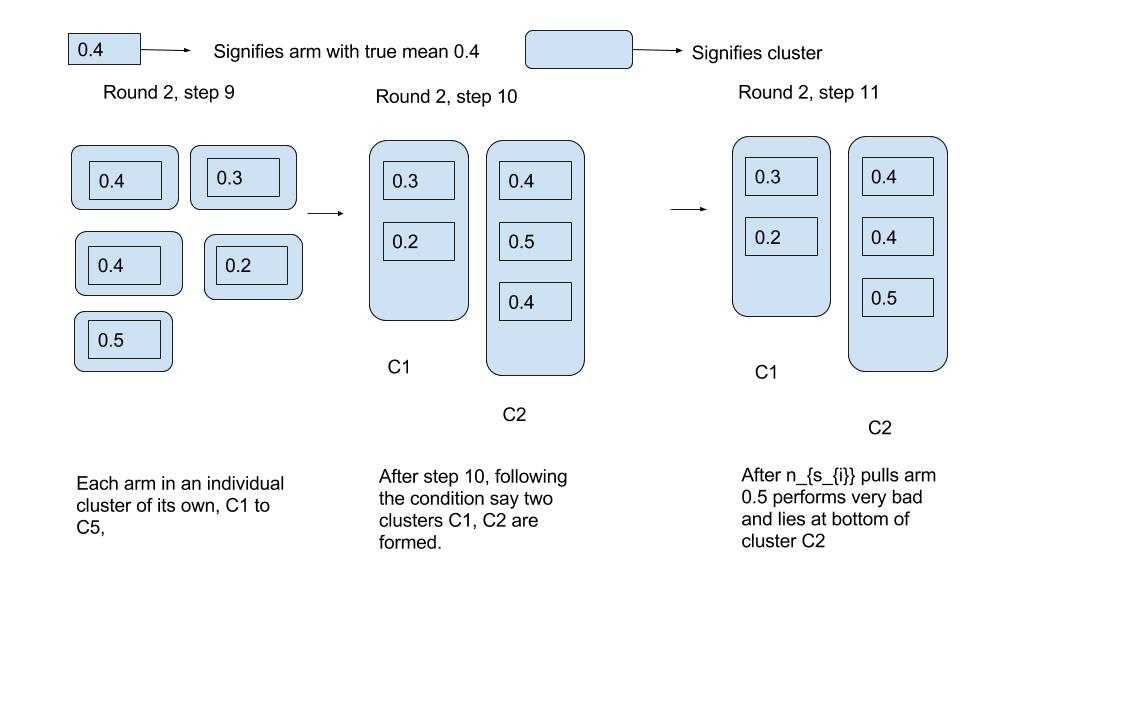
\includegraphics[scale=0.4]{img/diag1.jpg}
\caption{Steps 9-11}
\end{figure}
\begin{figure}[!tbp]
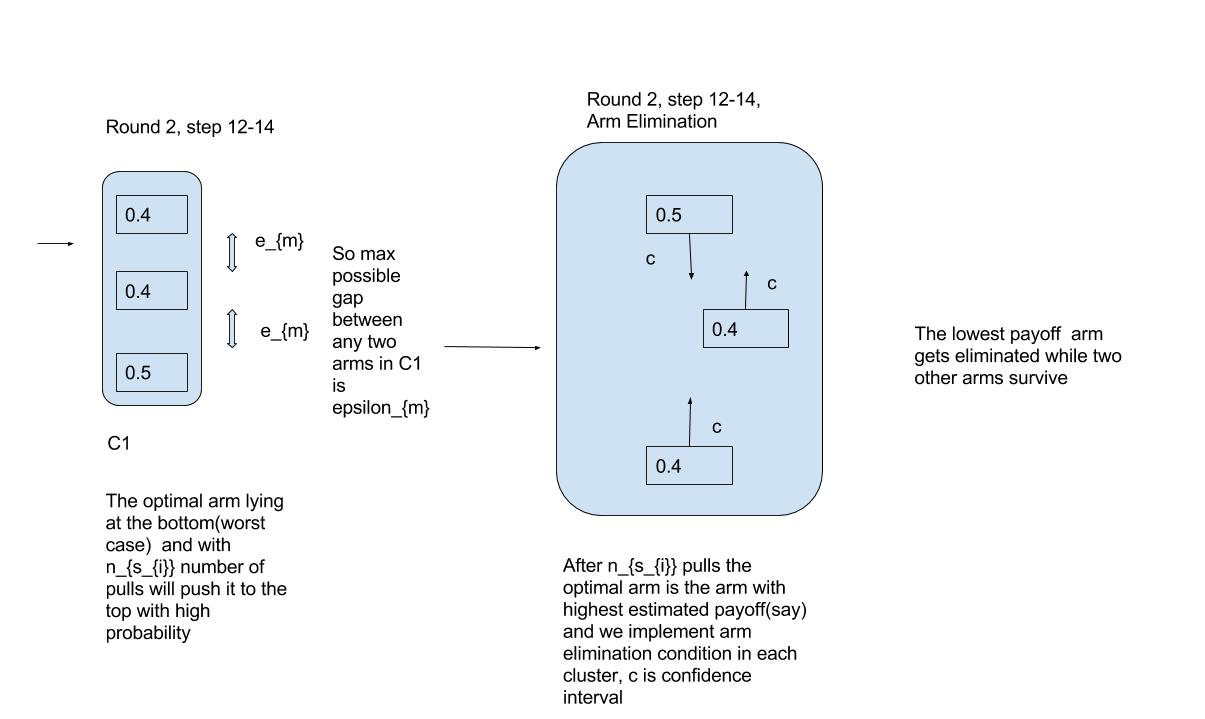
\includegraphics[scale=0.4]{img/diag2.jpg}
\caption{Steps 12-14}
\end{figure}
\begin{figure}[!tbp]
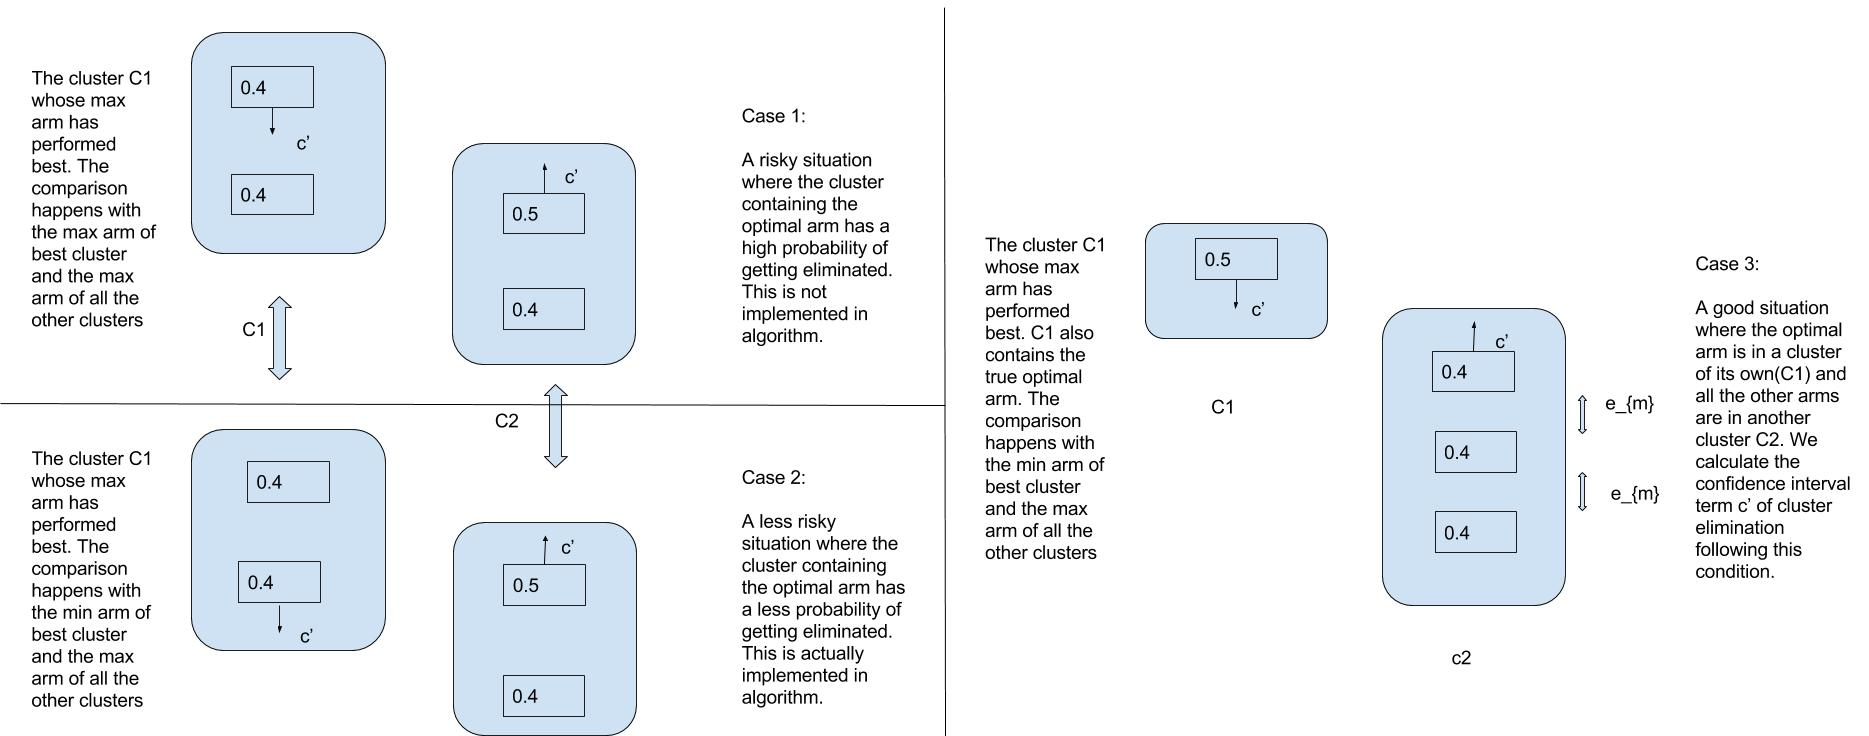
\includegraphics[scale=0.25]{img/diag3.jpg}
\caption{Different scenarios of Cluster Elimination}
\end{figure}




\section*{Appendix B}

\begin{proposition}
The number of times an arm $a_{i}\in s_{i}$ is pulled in each round is $n_{m}=\bigg\lceil\dfrac{2\log{(T\epsilon_{m}^{2})}}{\epsilon_{m}}\bigg\rceil$ and this eliminates the arm $a_{i}$ such that $\sqrt{\epsilon_{m}}<\dfrac{\Delta_{i}}{2}$ by the condition $\bigg\lbrace\hat{r}_{i} + \sqrt{\dfrac{\log (T\epsilon_{m}^{2})}{2w_{s_{i}} n_{m}}} < \max_{j\in s_{i}}\hat{r}_{j} - \sqrt{\dfrac{\log (T\epsilon_{m}^{2})}{2w_{s_{i}} n_{m}}} \bigg\rbrace, \forall s_{i}\in S$ with probability $\bigg\lbrace 1-\bigg(\dfrac{2}{T\epsilon_{m}^{2}}\bigg)\bigg\rbrace$. 
%where $B_{m}$ is the set of arms still not eliminated in the $m$-th round.
%- \sqrt{\dfrac{(\log{(4(\psi(m)T\epsilon_{m}^{2})}}{2w\ell_{m}n_{s_{i}}}}
\end{proposition}

\begin{proof} of Proposition 2:
\newline In arm elimination condition, given the choice of confidence interval $c_{m}$, we want to bound the event $\hat{r}_{i}+c_{m}\leq \hat{r}^{*}-c_{m}$. In this proof we will consider $w_{s_{i}}=1$ and $\psi(m)=1$. Later, we will discuss how different values of $w_{s_{i}}$ actually effects the regret bound.
%with a more tighter event of $ \hat{r}_{i} + \sqrt{w_{s_{i}}}c_{m} \leq \hat{r}^{*} - \sqrt{w_{s_{i}}}c_{m}$ which will result in faster elimination of arms within a cluster, given the choice of $c_{m}$ and $w_{s_{i}}$.
\newline Now, $c_{m}=\sqrt{\dfrac{\log (T\epsilon_{m}^{2})}{2 n_{m}}}$.
\newline Putting the value of $n_{m}=\dfrac{2\log{(T\epsilon_{m}^{2})}}{\epsilon_{m}}$ in $c_{m}$,
\newline $c_{m}=\sqrt{\dfrac{\epsilon_{m}\log (T\epsilon_{m}^{2})}{2*2 \log(T\epsilon_{m}^{2})}}=\dfrac{\sqrt{\epsilon_{m}}}{2} = \sqrt{\epsilon_{m+1}} < \dfrac{\Delta_{i}}{4} $
%\leq\dfrac{\epsilon_{m}\sqrt{\ell_{m}}}{2\sqrt{w\ell_{m}}}\leq \dfrac{\epsilon_{m}}{2\sqrt{w}}$.
%\newline But in $\xi_{1}$, $\ell_{m}=2^{m}$.
%\newline Hence, $c\leq \dfrac{\epsilon_{m} 2^{m/2}}{4}$.
\newline Again, $\exists a_{i} \in s_{i}$ such that, 
$\hat{r}_{i} + c_{m}\leq r_{i} + 2c_{m} $
%\newline\hspace*{14em}$= \hat{r}_{i}-\sqrt{\epsilon_{m}} + 2c_{m} +\sqrt{\epsilon_{m}}$
\newline\hspace*{14em}$= \hat{r}_{i} + 4c_{m} - 2c_{m} $
\newline\hspace*{14em}$\leq r_{i} + \Delta_{i} - 2c_{m}$
\newline\hspace*{14em}$< r^{*} -2c_{m} $
\newline\hspace*{14em}$\leq \hat{r}^{*} - c_{m}$
%\newline\hspace*{14em}$= r_{i} + 5\dfrac{\sqrt{\epsilon_{m}}}{\sqrt{w_{s_{i}}}} - 2\sqrt{w_{s_{i}}}c_{m}$
%\newline \hspace*{4em}
%\newline But, $\epsilon_{m}=\dfrac{\hat{\Delta}_{s,m}}{\ell_{m}}$, where $\hat{\Delta}_{s,m}=\max_{i\in B_{m}}{\hat{r}_{i}}-\min_{j\in B_{m}}{\hat{r}_{j}},i\neq j$ and $\ell_{m}$ is increased after every round.
%\newline \hspace*{4em}$\leq \hat{r}_{i} + \epsilon_{m} 2^{(m-4)/2} - 2c$
\newline Hence, we get that as soon as $\sqrt{\epsilon_{m}}<\dfrac{\Delta_{i}}{2}$, $\exists a_{i}\in s_{i}$ which gets eliminated.
%\newline So, $\hat{r}_{i}+c_{m}\leq \hat{r}_{i}+2c_{m}\leq r_{i} + \Delta_{i} - 2\sqrt{w_{s_{i}}}c_{m}\leq r^{*} - 2\sqrt{w_{s_{i}}}c_{m}$
%\leq \hat{r}^{*} - \sqrt{w}c_{m}
%\newline $\Rightarrow\hat{r}_{i}+c_{m}\leq \hat{r}_{i} - \sqrt{w}c_{m}  \leq r^{*} - \sqrt{w}c_{m}$
%\newline $\Rightarrow \hat{r}_{i} \leq {r}^{*} - 2\sqrt{w_{s_{i}}}c_{m} - 2c_{m} \leq \hat{r}^{*} - 2\sqrt{w_{s_{i}}}c_{m}$
\newline So, we need to bound the event of $\hat{r}_{i}+c_{m}\leq \hat{r}^{*}-c_{m}$ given that $\sqrt{\epsilon_{m}}<\dfrac{\Delta_{i}}{2}$ becomes true for some arm $a_{i}\in s_{i}$ after the $m$-th round and $c_{m}=\sqrt{\dfrac{\log (T\epsilon_{m}^{2})}{2 n_{m}}}$.
%\newline $\Rightarrow \hat{r}_{i}+2c_{m}\leq \hat{r}_{i} + 2\sqrt{w}c_{m} \leq \hat{r}^{*}$
%\newline $\Rightarrow \hat{r}_{i} + \sqrt{w}c_{m} \leq \hat{r}^{*} - \sqrt{w}c_{m}$
%\newline $\Rightarrow\hat{r}_{i}+c_{m}\sqrt{\dfrac{w\ell_{m}}{\epsilon_{m}}} \leq \hat{r}^{*}-c_{m}\sqrt{\dfrac{w\ell_{m}}{\epsilon_{m}}} $, as $c_{m}\sqrt{\dfrac{w\ell_{m}}{\epsilon_{m}}} > 0$

%\begin{proof} of Proposition 2:
%\newline
%Now, we can bound $\hat{r}_{i}+c_{m}\leq \hat{r}^{*}-c_{m}$ given that $\sqrt{\epsilon_{m}}<\dfrac{\Delta_{i}}{2}$ for some arm $a_{i}\in s_{i}$. 
	So, we need to bound the probability,
\newline\hspace*{4em} $\mathbb{P}\lbrace\hat{r}^{*}\leq r^{*} - c_{m}\rbrace\leq U_{m}$, where $U_{m}$ is an  arbitrary upper bound.
%, for a fixed $n_{s_{i}}$.
%\mathbb{P}\lbrace\hat{r}^{*}\leq r^{*} - c_{m}\rbrace\leq
\newline
%Here, we guarantee that only if $\hat{r}^{*}\leq r^{*} - c_{m}\sqrt{\dfrac{w\ell_{m}}{\epsilon_{m}}}$ or $\hat{r}_{i}\geq r_{i} + c_{m}\sqrt{\dfrac{w\ell_{m}}{\epsilon_{m}}}$ then only arm will not be deleted. This is a more aggressive arm elimination condition than simply looking at $\hat{r}^{*}\leq r^{*} - c_{m}$ or $\hat{r}_{i}\geq r_{i} + c_{m}$ because we are exploring much carefully by dividing the larger problem into sub-problems.
%\newline
Applying Chernoff-Hoeffding bound and considering independence of events,
\newline
\newline\hspace*{0em} $\mathbb{P}\lbrace\hat{r}^{*}\leq r^{*} - c_{m}\rbrace\leq exp(-2c_{m}^{2}n_{m})$
\newline\hspace*{2em} $\leq exp(-2 * \dfrac{\log (T\epsilon_{m}^{2})}{2 n_{m}} *n_{m})$
\newline\hspace*{2em} $\leq \dfrac{1}{T\epsilon_{m}^{2}}$
%$\leq \bigg(\dfrac{1}{4\psi(m)T\epsilon_{m}^{2}}\bigg)^{D}$, as $\ell_{m}-1\leq D$
%\newline\hspace*{2em}
\newline
Similarly, $\mathbb{P}\lbrace\hat{r}_{i}\geq r_{i} + c_{m}\rbrace\leq \dfrac{1}{T\epsilon_{m}^{2}}$
\newline
Summing, the two up, the probability that a sub-optimal arm $a_{i}$ is not eliminated in $m$-th round is  $\bigg(\dfrac{2}{T\epsilon_{m}^{2}}\bigg)$. 
\end{proof}

\todos{(Subho) Next part of the calculation mimicking UCB-Revisited is done in case 1 of Appendix D. }

\todos{(Subho) Appendix C, for Cluster Elimination is unchanged. We need to discuss. }

\section*{Appendix C}
\begin{proposition}
With a probability of $\bigg(1-\dfrac{4}{(\psi(m)T\epsilon_{m}^{2})^{1+|B_{m}|^{2}\epsilon_{m}}}\bigg)$ a sub-optimal arm can be deleted in round $m$, where $\hat{\Delta}_{m}=\max_{i\in B_{m}}{\lbrace\hat{r}_{i}\rbrace}-\min_{j\in B_{m}}{\lbrace\hat{r}_{j}\rbrace}$,  $\epsilon_{m}=\max{\bigg\lbrace\dfrac{\hat{\Delta}_{m}}{\ell_{m}}, \dfrac{1}{\sqrt{\psi{(m)T}}}\bigg\rbrace}$ for $\hat{\Delta}_{m}\neq 0$, $B_{m}$ is the set of arms still not eliminated in the $m$-th round and $T$ is the horizon.
\end{proposition}

\begin{proof} of Proposition 3:
\newline
Here, we will consider the scenario which will make it possible to remove all the arms in $B_{m}$ at one go. Let in the event $\xi_{2}$, there be two clusters $s_{i}$ and $s^{*}$ such that $a^{*}\in s^{*}$ and $a_{i}\in s_{i}, \forall a_{i}\setminus a^{*}\in B_{m}$. So, $|s^{*}|=1$ and $|s_{i}|=|B_{m}|-1\leq |B_{m}|$. Let $\hat{r}_{min_{s_{i}}}<\hat{r}_{i},\forall i\in s_{i}$ and $\hat{r}_{max_{s_{i}}}>\hat{r}_{i},\forall i\in s_{i}$ Thus, we see that if
\newline
\hspace*{2em} $\hat{r}_{max_{s_{i}}}+c_{m}' < \hat{r}^{*}-c_{m}' $, where $c_{m}'=\sqrt{\dfrac{|B_{m}|\epsilon_{m}\log{(\psi(m)T\epsilon_{m}^{2})}}{2\ell_{m} n_{m}}}$
\newline
then all the arms are eliminated and stopping condition reached. 
%In this $\xi_{2}$ we have to bound, 
%\newline
%\hspace*{4em}$\mathbb{P}\lbrace\hat{r}^{*}\leq \hat{r}_{s} + 2c_{m}\rbrace$
%\leq U_{m}$, where $U_{m}$ is an upper bound and $\hat{r}_{s}, \hat{r}_{b}\in s_{i}$
%\newline
We divide the proof into two parts. The above said event is the product of two simultaneous events, in the first event $\hat{r}_{max_{s_{i}}}+c_{m}' < \hat{r}^{*}-c_{m}'$ given that $\hat{r}_{max_{s_{i}}}>\hat{r}_{i}\forall i \in s_{i}$. In the first part we establish the probability of $\hat{r}_{max_{s_{i}}}+c_{m} < \hat{r}^{*}-c_{m}'$ just as before in Proposition 2. In the second the part we prove the bounds on the probability that $\exists a_{max_{s_{i}}}\in s_{i}$ such that $\hat{r}_{max_{s_{i}}}>\hat{r}_{i},\forall i \in s_{i}$ and $\sqrt{\epsilon_{m}}<\dfrac{2\Delta_{s}}{5}$ for the arm $a_{max_{s_{i}}}$ such that $\Delta_{s}=r^{*}-r_{max_{s_{i}}}=\Delta$ as $a_{s}$ is the arm that has the second highest $r_{s}$ after $r^{*}$ hence it lies closest to $a^{*}$.
\newline
Proceeding as like Proposition 2,
\newline
%$\hat{r}_{s}+c_{m}\leq \hat{r}_{s}+2\sqrt{w}c_{m}$, where $\sqrt{w}=\ell_{m}$
%\newline
\newline Now, for cluster elimination $c_{m}'=\sqrt{\dfrac{|B_{m}|\epsilon_{m}\log (\psi(m)T\epsilon_{m}^{2})}{2\ell_{m} n_{m}}}$
%, where $w=\dfrac{\ell_{m}}{|B_{m}|}$
\newline Putting the value of $n_{m}=\dfrac{2\log{(\psi(m)T\epsilon_{m}^{2})}}{\epsilon_{m}}$ in $c_{m}'$,
\newline $c_{m}'=\sqrt{\dfrac{\epsilon_{m}^{2}|B_{m}|\log (\psi(m)T\epsilon_{m}^{2})}{2\ell_{m}*2 \log(\psi(m)T\epsilon_{m}^{2})}}=\dfrac{\epsilon_{m}\sqrt{|B_{m}|}}{2\sqrt{\ell_{m}}}$
%\leq\dfrac{\epsilon_{m}\sqrt{\ell_{m}}}{2\sqrt{w\ell_{m}}}\leq \dfrac{\epsilon_{m}}{2\sqrt{w}}$.
%\newline But in $\xi_{1}$, $\ell_{m}=2^{m}$.
%\newline Hence, $c\leq \dfrac{\epsilon_{m} 2^{m/2}}{4}$.
\newline Again, we know that $\ell_{m}\geq |B_{m}|-1$ and $\dfrac{\ell_{m}}{|B_{m}|\epsilon_{m}}=\dfrac{\ell_{m}^{2}}{|B_{m}|\Delta_{m}}$ and so $\dfrac{\ell_{m}}{|B_{m}|\epsilon_{m}}\geq 1$.
\newline Again, $\exists a_{max_{s_{i}}} \in s_{i}$ such that, 
$\hat{r}_{max_{s_{i}}} + c_{m}'\leq \hat{r}_{max_{s_{i}}} + 2c_{m}'$, as $c_{m}' > 0$
\newline\hspace*{14em}$\leq\hat{r}_{max_{s_{i}}} + 2\sqrt{\dfrac{\ell_{m}}{|B_{m}|\epsilon_{m}}}c_{m}' $
\newline\hspace*{14em}$\leq r_{max_{s_{i}}} + 3\sqrt{\dfrac{\ell_{m}}{|B_{m}|\epsilon_{m}}}c_{m}'$
\newline\hspace*{14em}$\leq r_{max_{s_{i}}} + 5\sqrt{\dfrac{\ell_{m}}{|B_{m}|\epsilon_{m}}}c_{m}'-\sqrt{\dfrac{\ell_{m}}{|B_{m}|\epsilon_{m}}}c_{m}'$
\newline\hspace*{14em}$\leq r_{max_{s_{i}}} + 5\dfrac{\sqrt{\epsilon_{m}}}{2}-\sqrt{\dfrac{\ell_{m}}{|B_{m}|\epsilon_{m}}}c_{m}'$
%\newline\hspace*{14em}$\leq r_{s} + 5\dfrac{\epsilon_{m}}{2}-\sqrt{\dfrac{\ell_{m}}{|B_{m}|\epsilon_{m}}}c_{m}'$
%\leq r_{s} + 2\dfrac{\epsilon_{m}}{\sqrt{w}}-\sqrt{\dfrac{\ell_{m}}{|B_{m}|\epsilon_{m}}}c_{m}'$
%$\leq r_{s} - 2\sqrt{w}c_{m}' + 10\dfrac{\sqrt{\epsilon_{m}}}{2\sqrt{w}} \leq r_{i} + 5\dfrac{\sqrt{\epsilon_{m}}}{\sqrt{w}} - 2\sqrt{w}c_{m}'$
\newline Also in $\xi_{2}$, $\sqrt{\epsilon_{m}}<\dfrac{2\Delta_{s}}{5}$, $\exists a_{max_{s_{i}}}\in s_{i}$
\newline We can immediately see that the condition in $\xi_{2}$ happens after $\xi_{1}$ because $\sqrt{\dfrac{\epsilon_{m}}{w_{s_{i}}}}<\dfrac{\Delta_{i}}{5}$ will occur before $\sqrt{\epsilon_{m}}<\dfrac{2\Delta_{s}}{5}$ with a higher probability given the value of $w_{s_{i}}\geq 4$. Hence, $w_{s_{i}}=\ell_{m}^{2}k_{s_{i}}$ guarantees that $\xi_{2}$ happens after $\xi_{1}$ with high probability.
\newline
$\hat{r}_{max_{s_{i}}} + 2c_{m}'\leq\hat{r}_{max_{s_{i}}} + 2\sqrt{\dfrac{\ell_{m}}{|B_{m}|\epsilon_{m}}}c_{m}'\leq r_{max_{s_{i}}} + \Delta_{s}-\sqrt{\dfrac{\ell_{m}}{|B_{m}|\epsilon_{m}}}c_{m}'$
\newline\hspace*{14em}$\leq r^{*}-\sqrt{\dfrac{\ell_{m}}{|B_{m}|\epsilon_{m}}}c_{m}'$
\newline\hspace*{14em}$\leq \hat{r}^{*}$
\newline
So, from the condition imposed in $\xi_{2}$, given that $\exists a_{i}\in s_{i}$ such that $\sqrt{\epsilon_{m}}<\dfrac{2\Delta_{s}}{5}$ for the given $c_{m}'$, we will be upper bounding the probability of $\hat{r}_{max_{s_{i}}} + 2c_{m}'\leq\hat{r}^{*}$ with $\hat{r}_{max_{s_{i}}} + 2\sqrt{\dfrac{\ell_{m}}{|B_{m}|\epsilon_{m}}}c_{m}'\leq \hat{r}^{*}\Rightarrow\hat{r}_{max_{s_{i}}} + \sqrt{\dfrac{\ell_{m}}{|B_{m}|\epsilon_{m}}}c_{m}'\leq \hat{r}^{*}-\sqrt{\dfrac{\ell_{m}}{|B_{m}|\epsilon_{m}}}c_{m}'$.
\newline
Applying Chernoff-Hoeffding bound and considering independence of events,
\newline
$\mathbb{P}\lbrace\hat{r}^{*}\leq r^{*} - \sqrt{\dfrac{\ell_{m}}{|B_{m}|\epsilon_{m}}}c_{m}'\rbrace\leq exp(-2*(\sqrt{\dfrac{\ell_{m}}{|B_{m}|\epsilon_{m}}}c_{m}')^{2}n_{m})=\dfrac{1}{ (\psi(m)T\epsilon_{m}^{2})}$
\newline
Similarly, $\mathbb{P}\lbrace\hat{r}_{max_{s_{i}}}\geq r_{max_{s_{i}}} - \sqrt{\dfrac{\ell_{m}}{|B_{m}|\epsilon_{m}}}c_{m}'\rbrace\leq\dfrac{1}{ (\psi(m)T\epsilon_{m}^{2})}$
%\mathbb{P}\lbrace\hat{r}^{*}\leq \hat{r}_{b} + |B_{m}-2|\epsilon_{m} + 2c_{m}\rbrace\leq\mathbb{P}\lbrace\hat{r}^{*}\leq \hat{r}_{b} + |B_{m}|\epsilon_{m} + 2c_{m}\rbrace$
%=\mathbb{P}\lbrace\hat{r}^{*}\leq \hat{r}_{s} - |B_{m}|\epsilon_{m} - c\rbrace
\newline Now, for bounding the event that for the arm $a_{max_{s_{i}}}\in s_{i}$, $\hat{r}_{max_{s_{i}}}\geq \hat{r}_{i}, \forall i\in s_{i}$ and also $a_{min_{s_{i}}}$ be an arm such that $\hat{r}_{min_{s_{i}}}< \hat{r}_{i}, \forall i\in s_{i}$
\newline
$\mathbb{P}\lbrace\hat{r}_{max_{s_{i}}}\geq \hat{r}_{i}|\forall i\in s_{i}\rbrace\leq \mathbb{P}\lbrace\hat{r}_{max_{s_{i}}}\geq \hat{r}_{min_{s_{i}}}+(|B_{m}|-2)\epsilon_{m}\rbrace\leq \mathbb{P}\lbrace\hat{r}_{max_{s_{i}}} \geq \hat{r}_{min_{s_{i}}}+|B_{m}|\epsilon_{m}\rbrace$
\newline
$\Rightarrow \mathbb{P}\lbrace \hat{r}_{max_{s_{i}}} - \dfrac{|B_{m}|\epsilon_{m}}{2} \geq \hat{r}_{min_{s_{i}}}+\dfrac{|B_{m}|\epsilon_{m}}{2} \rbrace$
%\newline
%$\Rightarrow\mathbb{P}\lbrace\hat{r}^{*}-\dfrac{|B_{m}|\epsilon_{m} + 2c_{m}}{2}\leq \hat{r}_{b} + \dfrac{|B_{m}|\epsilon_{m} + 2c_{m}}{2}\rbrace$
%%But, in $\xi_{2}$, we know that $\hat{r}_{s}\leq\hat{r}^{*}$ and let $\hat{r}^{*}\geq r^{*}$.
%\newline
%$\Rightarrow \mathbb{P}\lbrace\hat{r}^{*}\leq r^{*} - \dfrac{(|B_{m}|\epsilon_{m} + 2c_{m})}{2}\rbrace\leq \mathbb{P}\lbrace\hat{r}^{*}\leq r^{*} - \sqrt{\dfrac{|B_{m}|w }{\epsilon_{m}}}c_{m}\rbrace$ as $\sqrt{\dfrac{|B_{m}|w }{\epsilon_{m}}}c_{m} > \dfrac{(|B_{m}|\epsilon_{m} + 2c_{m})}{2}$
\newline
Again applying Chernoff-Hoeffding bound and considering independence of events,
\newline
$\mathbb{P}\lbrace\hat{r}_{max_{s_{i}}}\leq r_{max_{s_{i}}} - \dfrac{|B_{m}|\epsilon_{m}}{2}\rbrace\leq exp(-2*(\dfrac{|B_{m}|\epsilon_{m}}{2})^{2}n_{m})\leq exp\bigg(-2*(\dfrac{|B_{m}|\epsilon_{m}}{2})^{2}\dfrac{2\log{(\psi(m)T\epsilon_{m}^{2})}}{\epsilon_{m}}\bigg)$
\newline\hspace*{21em}$\leq \bigg(\dfrac{1}{(\psi(m)T\epsilon_{m}^{2})^{|B_{m}|^{2}\epsilon_{m}}}\bigg)$
%\newline
%$\mathbb{P}\lbrace\hat{r}^{*}\leq \hat{r}_{s} - (|B_{m}|\epsilon_{m} + c)\rbrace\leq exp(-2*((|B_{m}|\epsilon_{m} + c)^{2}n_{s_{i}})$
%\newline Now, $(\dfrac{|B_{m}|\epsilon_{m} + c_{m}}{2})^{2} \geq \dfrac{w\ell_{m}}{|B_{m}|}\dfrac{c_{m}^{2}}{\epsilon_{m}}$, in $\xi_{2}$ for sufficiently large $|B_{m}|\leq K$
%\newline Now, $(|B_{m}|\epsilon_{m} + c)^{2} \geq \dfrac{c^{2}}{\epsilon_{m}}$, in $\xi_{2}$ for sufficiently large $B_{m}\leq K$.
%\newline $\mathbb{P}\lbrace\hat{r}^{*}\leq r^{*} - \sqrt{\dfrac{|B_{m}|w }{\epsilon_{m}}}c_{m}\rbrace\leq exp(-2*\dfrac{|B_{m}|w\epsilon_{m}\log{(4\psi(m)T\epsilon_{m}^{2})}}{2w|B_{m}| n_{s_{i}}\epsilon_{m}}n_{s_{i}})$
%\newline\hspace*{4em} $\leq exp(-\dfrac{|B_{m}|\log{(4\psi(m)T\epsilon_{m}^{2})}}{(w)})\leq \dfrac{1}{(4\psi(m)T\epsilon_{m}^{2})^{|B_{m}|/(w\ell_{m})}}\leq \bigg(\dfrac{1}{4(\psi(m)T\epsilon_{m}^{2}}\bigg)^{|B_{m}|/w\ell_{m}}$
\newline Similarly, $\mathbb{P}\lbrace\hat{r}_{min_{s_{i}}}\geq r_{min_{s_{i}}} + \dfrac{|B_{m}|\epsilon_{m}}{2}\rbrace\leq \bigg(\dfrac{1}{(\psi(m)T\epsilon_{m}^{2})^{|B_{m}|^{2}\epsilon_{m}}}\bigg)$
\newline Considering two events and from the conditions imposed in $\xi_{2}$ and the stopping condition in the algorithm, we can see that the probability of the set $s_{i}$ not getting deleted and the rounds not stopping is given by,
\newline
\hspace*{2em}$\bigg(\dfrac{2}{\psi(m)T\epsilon_{m}^{2}}\bigg)\times\bigg(\dfrac{2}{(\psi(m)T\epsilon_{m}^{2})^{|B_{m}|^{2}\epsilon_{m}}}\bigg)=\bigg(\dfrac{4}{(\psi(m)T\epsilon_{m}^{2})^{1+|B_{m}|^{2}\epsilon_{m}}}\bigg)$.
%\newline Thus, from the conditions imposed on $\xi_{1}$ and $\xi_{2}$ we see that the cluster deletion condition is a tighter elimination condition than arm elimination condition. This is because for cluster elimination the condition depends on the number of arms surviving till $m$-th round that is $|B_{m}|$ which itself depends on the exploration $n_{s_{i}}$ and cluster size limit $D$.
\end{proof}

\section*{Appendix D}
\begin{theorem}
The upper bound on the total regret over horizon $T$ after round $m$ is given by $R_{T}\leq \sum_{i\in A}\bigg (\max{\bigg\lbrace \bigg(\dfrac{27}{c(\Delta_{i})^{\frac{3}{5}}}\bigg) ,\bigg(\dfrac{25\Delta_{i}}{c\Delta^{2})(0.16cT\Delta^{2})^{2\Delta/5}}\bigg)\bigg\rbrace} + \bigg(\Delta_{i}+\dfrac{27\log{(cT\dfrac{\Delta_{i}^{\frac{8}{5}}}{12})}}{\Delta_{i}^{\frac{3}{5}}}\bigg)\bigg)$, where $c>0$ is a constant, $A$ is the set of arms and $\Delta$ is the minimal gap.
\end{theorem}

\todos{(Subho) Case 1 is case(a) and Case 2 is case(b1) in UCB-Revisited Proof}

\begin{proof} of Theorem 1: 
\subsubsection{Case 1:}
Given that in round $m$, either a sub-optimal arm $a_{i}\in s_{i}$ gets eliminated or the cluster $s_{i}$ itself will get eliminated. So, for an arm $a_{i}$ to survive, both these events should fail to delete the arm. In round $m$, the regret suffered for not eliminating an arm $a_{i}$ is given by,
\newline
\hspace*{1em} $\max{\bigg\lbrace \bigg(\dfrac{2}{T\epsilon_{m}^{2}}\bigg) ,\bigg(\dfrac{4}{(\psi(m)T\epsilon_{m}^{2})^{1+|B_{m}|^{2}\epsilon_{m}}}\bigg)\bigg\rbrace}$ ~~~~~~~~~~~~~~~~ (1)
\newline
\newline from \textbf{section 4, Proposition 2 and section 4, Proposition 3}.
\newline
Now, that an arm gets eliminated within a cluster if $\sqrt{\epsilon_{m}}<\dfrac{\Delta_{i}}{2}$ and also we know that all arms get eliminated within a cluster if $\exists a_{max_{s_{i}}}\in s_{i}$ such that $\sqrt{\epsilon_{m}}<\dfrac{2\Delta_{s}}{5}$ and $\hat{r}_{max_{s_{i}}}>\hat{r}_{i},\forall i\in s_{i}$. So, if $\sqrt{\epsilon_{m}}<\dfrac{\Delta_{i}}{2}$ and $\sqrt{\epsilon_{m}}\geq\dfrac{2\Delta_{s}}{5}$ in $\xi_{2}$ then we can say that arm $a_{i}$ will not be eliminated. 
\newline
%Extending, from previous inequality if $\epsilon_{m}\geq \sqrt{\epsilon_{m}}\geq\dfrac{\sqrt{w}\Delta_{i}}{5}$ in $\xi_{1}$ or if $\epsilon_{m}\geq\sqrt{\epsilon_{m}}\geq\dfrac{2\Delta_{s}}{5}$ then arm $a_{i}$ will not be eliminated. 
%\newline
%Again, in $\xi_{1}$ when arm $a_{i}$ is eliminated, we can tightly bound $\epsilon_{m}$ such that,
%\newline
%$\sqrt{\dfrac{\epsilon_{m}}{w_{s_{i}}}}\leq\dfrac{\Delta_{i}}{5}\Rightarrow \sqrt{\dfrac{\epsilon_{m}}{\ell_{m}^{3}}}\leq\dfrac{\Delta_{i}}{5}$, as $w_{s_{i}}\leq \ell_{m}^{3}$
%\newline 
%\hspace*{5em}$\Rightarrow \sqrt{\dfrac{\epsilon_{m}}{D_{m}^{3}}}\leq\dfrac{\Delta_{i}}{5}$, since $\ell_{m}\leq D_{m}$
%\newline
%\hspace*{5em}$\Rightarrow \sqrt{\dfrac{\epsilon_{m}}{(1/\sqrt{\epsilon_{m}})^{3}}}\leq\dfrac{\Delta_{i}}{5}$, since $D_{m}=\dfrac{1}{\sqrt{\epsilon_{m}}}$
%\newline
%\hspace*{5em}$\Rightarrow \epsilon_{m}\leq(\dfrac{\Delta_{i}}{5})^{\frac{4}{5}}$
%\newline
%Hence, in the $m$-th round if $\epsilon_{m}\geq(\dfrac{\Delta_{i}}{5})^{\frac{4}{5}}$, we can definitely say that arm $a_{i}$ is not eliminated in $\xi_{1}$.
%\newline
%Proceeding similarly in $\xi_{2}$, we know that,
%\newline
%$\sqrt{\epsilon_{m}}\leq\dfrac{2\Delta_{s}}{5}\Rightarrow \dfrac{\sqrt{\epsilon_{m}}}{\ell_{m}}\leq\dfrac{2\Delta_{s}}{5}$ 
%\newline 
%\hspace*{5em}$\Rightarrow \dfrac{\sqrt{\epsilon_{m}}}{D_{m}}\leq\dfrac{2\Delta_{s}}{5}$, since $\ell_{m}\leq D_{m}$
%\newline
%\hspace*{5em}$\Rightarrow \epsilon_{m}\leq\dfrac{2\Delta_{s}}{5}$, since $D_{m}=\dfrac{1}{\sqrt{\epsilon_{m}}}$
%%\newline
%%\hspace*{5em}$\Rightarrow \epsilon_{m}\leq(\dfrac{\Delta_{i}}{5})^{\frac{4}{5}}$
%\newline
%Hence, in the $m$-th round if $\epsilon_{m}\geq\dfrac{2\Delta_{s}}{5}$, a cluster $s_{i}$, such that $\exists a_{max_{s_{i}}}\in s_{i}$ and $\hat{r}_{max_{s_{i}}}\geq\hat{r}_{i},\forall i\in s_{i}$, then $s_{i}$ is not eliminated in $\xi_{2}$.
%\newline
Bounding equation (1) trivially by  $T\Delta_{i}$,
\newline\newline
$\Rightarrow \max{\bigg\lbrace \bigg(\dfrac{2T\Delta_{i}}{T\epsilon_{m}^{2}}\bigg) ,\bigg(\dfrac{4T\Delta_{i}}{(\psi(m)T\epsilon_{m}^{2})^{1+|B_{m}|^{2}\epsilon_{m}}}\bigg)\bigg\rbrace}$
\newline
$\leq \max{\bigg\lbrace \bigg(\dfrac{2\Delta_{i}}{(\dfrac{\Delta_{i}}{2})^{4}\bigg)} ,\bigg(\dfrac{4T\Delta_{i}}{(\psi(m)T\dfrac{4\Delta_{s}^{2}}{25})\times(\psi(m)T\dfrac{4\Delta_{s}^{2}}{25})^{|B_{m}|^{2}\epsilon_{m}}}\bigg)\bigg\rbrace}$
\newline
$\leq \max{\bigg\lbrace \bigg(\dfrac{32\Delta_{i}}{(\Delta_{i})^{4}}\bigg) ,\bigg(\dfrac{25\Delta_{i}}{(\psi(m)\Delta_{s}^{2})\times(0.16\psi(m)T\Delta_{s}^{2})^{|B_{m}|^{2}2\Delta_{s}/5}}\bigg)\bigg\rbrace}$
\newline
$\leq \max{\bigg\lbrace \bigg(\dfrac{32}{(\Delta_{i})^{3}}\bigg) ,\bigg(\dfrac{25\Delta_{i}}{(\psi(m)\Delta_{s}^{2})\times(0.16\psi(m)T\Delta_{s}^{2})^{2|B_{m}|^{2}\Delta_{s}/5}}\bigg)\bigg\rbrace}$
\newline
$\leq \max{\bigg\lbrace \bigg(\dfrac{32}{(\Delta_{i})^{3}}\bigg) ,\bigg(\dfrac{25\Delta_{i}}{(\psi(m)\Delta^{2})(0.16\psi(m)T\Delta^{2})^{2|B_{m}|^{2}\Delta/5}}\bigg)\bigg\rbrace}$, as $\Delta_{s}\geq \Delta$
%\newline
%$\leq \max{\bigg\lbrace \bigg(\dfrac{1250}{2^{4}\psi(m)\Delta_{i}^{3})}\bigg) ,\bigg(\dfrac{625\Delta_{i}}{(\psi(m)\Delta^{4})\times(39\psi(m)T \Delta^{4})^{2|B_{m}|^{2}\Delta_{s}/5}}\bigg)\bigg\rbrace}$, as $\ell_{m}\geq 2$
%\newline
%$\leq \max{\bigg\lbrace \bigg(\dfrac{79}{\psi(m)\Delta_{i}^{3})}\bigg) ,\bigg(\dfrac{625\Delta_{i}}{(\psi(m)\Delta^{4})\times(39\psi(m)T\Delta^{4})^{|B_{m}|^{2}\epsilon_{m}}}\bigg)\bigg\rbrace}$, since $\epsilon_{m}<\Delta_{max}$
%\newline
%\newline$\leq \max{\bigg\lbrace \bigg(\dfrac{16\Delta_{i}T}{(4\psi(m)T\epsilon_{m}^{2})^{D}}\bigg),\bigg(\dfrac{16\Delta_{i}T}{(4\psi(m)T\epsilon_{m}^{2})^{|B_{m}|D}}\bigg)\bigg\rbrace}$
Hence, total regret till round $m$ is,
\newline
$\leq \max{\bigg\lbrace \bigg(\dfrac{32}{(\Delta_{i})^{3}}\bigg) ,\bigg(\dfrac{25\Delta_{i}}{(\psi(m)\Delta^{2})(0.16\psi(m)T\Delta^{2})^{2|B_{m}|^{2}\Delta/5}}\bigg)\bigg\rbrace}$
\newline
Summing over all arms left till round $m$,
\newline
$\leq \sum_{i\in B_{m}}\max{\bigg\lbrace \bigg(\dfrac{32}{(\Delta_{i})^{3}}\bigg),\bigg(\dfrac{25\Delta_{i}}{(\psi(m)\Delta^{2})(0.16\psi(m)T\Delta^{2})^{2|B_{m}|^{2}\Delta/5}}\bigg)\bigg\rbrace}$, 
%\newline
\subsubsection{Case 2:}
Again, from \textbf{section 4, Proposition 1}, we know that given the arm $a_{i}\in s_{i}$ has survived till this round, $a_{i}$ got pulled $n_{m}$ number of times from $1,2,..,m$ and so the regret suffered due to $a_{i}$ is no less than,
\newline
\hspace*{4em}$n_{m}=\bigg\lceil\dfrac{2\log{(T\epsilon_{m}^{2})}}{\epsilon_{m}}\bigg\rceil$
\newline
Also, since we are exploring locally within a cluster and an arm is pulled no longer till it is eliminated by the arm elimination rule, 
%\newline
%$\sqrt{\dfrac{\epsilon_{m}}{w}}<\dfrac{\Delta_{i}}{5}\Rightarrow \sqrt{\dfrac{\epsilon_{m}}{\ell_{m}^{2}}}<\dfrac{\Delta_{i}}{5}$, as $w\geq \ell_{m}^{2}$
%\newline
%$\Rightarrow \sqrt{\dfrac{\epsilon_{m}}{\ell_{m}^{2}}}<\dfrac{\Delta_{i}}{5}$
%\newline
So, the total contribution of $a_{i}$  till round $m$ is given by,
\newline
\hspace*{4em}$\Delta_{i}\bigg\lceil\dfrac{2\log{(T\epsilon_{m}^{2})}}{\epsilon_{m}}\bigg\rceil$
%\newline
%\hspace*{4em}
$\leq\Delta_{i}\bigg\lceil\dfrac{2\log{(T(\dfrac{\Delta_{i}}{2})^{4})}}{(\dfrac{\Delta_{i}}{2})^{4}}\bigg\rceil$, since $\sqrt{\epsilon_{m}}\leq\dfrac{\Delta_{i}}{2}$
\newline
\hspace*{14em}
$\leq\Delta_{i}\bigg(1+\dfrac{32\log{(T(\dfrac{\Delta_{i}}{2})^{4})}}{\Delta_{i}^{2}}\bigg)$
\newline
\hspace*{14em}
$\leq\Delta_{i}\bigg(1+\dfrac{32\log{(T\dfrac{\Delta_{i}^{4}}{16})}}{\Delta_{i}^{2}}\bigg)$
\newline
Summing over all arms left till round $m$,
\newline
\hspace*{4em}$\leq\sum_{i\in B_{m}}\Delta_{i}\bigg(1+\dfrac{32\log{(T\dfrac{\Delta_{i}^{4}}{12}})}{\Delta_{i}^{2}}\bigg)$
\newline
%\hspace*{4em}$\leq\sum_{i\in B_{m}}\bigg(\Delta_{i}+\dfrac{27\log{(\psi(m)T\dfrac{\Delta_{i}^{\frac{8}{5}}}{12})}}{\Delta_{i}^{\frac{3}{5}}}\bigg)$
%\newline
%\hspace*{4em}$\leq\sum_{i\in B_{m}}\bigg(\Delta_{i}+\dfrac{12.5\log{(\psi(m)T\Delta_{i}^{4})}}{\Delta_{i}}\bigg)$
	%Thus, we see that the growth of the $n_{s_{i}}$ is always linear and not quadratic as in UCB-Revisited(\cite{auer2010ucb}). Also once $2l_{m}=D$, then $n_{s_{i}}$ will remain constant for the next rounds till stopping condition is met. Thus we have a more controlled exploration than UCB-Revisited(\cite{auer2010ucb}) and Median Elimination(\cite{even2006action}). Hence, 
%\newline
%\hspace*{4em}$\leq\sum_{i\in B_{m}}\bigg(\Delta_{i}+\dfrac{54\log{(\psi(m)T\dfrac{\Delta_{i}^{\frac{8}{5}}}{12})}}{\Delta_{i}^{\frac{3}{5}}}\bigg)$
\newline
Summing up \textbf{Case 1} and \textbf{Case 2}, the total regret till round $m$ is given by,
\newline $R_{T}\leq \sum_{i\in B_{m}}\bigg (\max{\bigg\lbrace \bigg(\dfrac{32}{(\Delta_{i})^{3}}\bigg) ,\bigg(\dfrac{25\Delta_{i}}{(\psi(m)\Delta^{2})(0.16\psi(m)T\Delta^{2})^{2|B_{m}|^{2}\Delta/5}}\bigg)\bigg\rbrace} + \bigg(\Delta_{i}+\dfrac{32\log{(T\dfrac{\Delta_{i}^{4}}{16})}}{\Delta_{i}}\bigg)\bigg)$
\newline
%But, $\psi(m)\leq c/m$ for any $c>0$ and so the regret upper bound comes off as 
But, $\psi(m) = 1$ the regret upper bound comes off as 
\newline
$R_{T}\leq \sum_{i\in B_{m}}\bigg (\max{\bigg\lbrace \bigg(\dfrac{32}{(\Delta_{i})^{3}}\bigg) ,\bigg(\dfrac{25\Delta_{i}}{(\Delta^{2})(0.16T\Delta^{2})^{2|B_{m}|^{2}\Delta/5}}\bigg)\bigg\rbrace} + \bigg(\Delta_{i}+\dfrac{32\log{(T\dfrac{\Delta_{i}^{4}}{16})}}{\Delta_{i}}\bigg)\bigg)$.

\end{proof}

\todos{(Subho) Sir I want to point out an important thing here. What we derived is actually a single instance of UCB-Revisited. But actually we are not running a single instance but multiple instances(as many number as the clusters) of UCB-Revisited. That's why it performing good and also that was the initial intuition. So we need to find some way to incorporate this in our proof.}


\section*{Appendix E}
\begin{theorem}
The error bound till round $m$ is given by $e_{t}\leq \sum_{i\in A^{'}}\bigg(\dfrac{51}{\psi(m)\Delta_{i}^{6/5}} \bigg)+\sum_{i\in A^{''}\setminus A^{'}}\bigg(\dfrac{51}{\psi(m)\Delta_{b}^{6/5}} \bigg)$, where the arms surviving till $m$-th round belong to the set $A^{'}$, arms to still survive and eliminate arm $a^{*}$ after round $m$ belong to $A^{''}$.
\end{theorem}
\begin{proof} of Theorem 2
\newline
Let,  $\xi_{3}$ be the event that the optimal arm $a^{*}$ was eliminated by a sub-optimal arm. In any round $m_{*}$, if the optimal arm $a^{*}$ gets eliminated then for any round from $1$ to $m_{j}$ all arms $a_{j}$ such that $\sqrt{\dfrac{\epsilon_{m}}{w_{s_{i}}}}<\dfrac{\Delta_{i}}{5}$ were eliminated. Let, the arms surviving till $m_{*}$ round be denoted by $A^{'}$. This leaves any arm $a_{b}$ such that $\sqrt{\dfrac{\epsilon_{m}}{w_{s_{i}}}}>\dfrac{\Delta_{b}}{5}$ to still survive and eliminate arm $a^{*}$ in round $m_{*}$. Let, such arms that survive $a^{*}$ belong to $A^{''}$. Also maximal regret per step after eliminating $a^{*}$ is the maximal $\Delta_{j}$ among the remaining arms $a_{j}$ with $m_{j}\geq m_{*}$.  Let $m_{b}$ be the round when $\sqrt{\dfrac{\epsilon_{m}}{w_{s_{i}}}}<\dfrac{\Delta_{b}}{5}$. Hence, the maximal regret after eliminating the arm $a^{*}$ is upper bounded by, 
\newline
$\sum_{m_{*}=0}^{max_{j\in A^{'}}m_{j}}\sum_{i\in A^{''}:m_{i}>m_{*}}\bigg(\dfrac{2}{\psi(m)T\epsilon_{m}^{2}} \bigg).T\max_{j\in A^{''}:m_{j}\geq m_{*}}{\Delta}_{j}$
\newline
\hspace*{0em}$\leq\sum_{m_{*}=0}^{max_{j\in A^{'}}m_{j}}\sum_{i\in A^{''}:m_{i}>m_{*}}\bigg(\dfrac{2}{\psi(m)T\epsilon_{m}^{2}} \bigg).T.5\sqrt{\dfrac{\epsilon_{m}}{w_{s_{i}}}}$, since $\sqrt{\dfrac{\epsilon_{m}}{w_{s_{i}}}}<\dfrac{\Delta_{i}}{5}$
\newline
\hspace*{0em}$\leq\sum_{m_{*}=0}^{max_{j\in A^{'}}m_{j}}\sum_{i\in A^{''}:m_{i}>m_{*}}\dfrac{10}{2}\bigg(\dfrac{1}{\psi(m)\epsilon_{m}^{3/2}} \bigg) $, as $w_{s_{i}}\geq 4$
\newline
\hspace*{0em}$\leq\sum_{m_{*}=0}^{max_{j\in A^{'}}m_{j}}\sum_{i\in A^{''}:m_{i}>m_{*}}\bigg(\dfrac{14}{\psi(m)\Delta_{i}^{6/5}} \bigg) $, as $\epsilon_{m}\geq(\dfrac{\Delta_{i}}{5})^{\frac{4}{5}}$
\newline
\hspace*{0em}$\leq\sum_{i\in A^{''}:m_{i}>m_{*}}\sum_{m_{*}=0}^{\min{\lbrace m_{i},m_{b}\rbrace}}\bigg(\dfrac{14}{\psi(m)\Delta_{i}^{6/5}} \bigg) $
\newline
\hspace*{0em}$\leq\sum_{i\in A^{'}}\bigg(\dfrac{14}{\psi(m)\Delta_{i}^{6/5}} \bigg)+\sum_{i\in A^{''}\setminus A^{'}}\bigg(\dfrac{14}{\psi(m)\Delta_{b}^{6/5}} \bigg)$
\newline
\hspace*{0em}$\leq\sum_{i\in A^{'}}\bigg(\dfrac{14*5^{4/5}}{\psi(m)\Delta_{i}^{6/5}} \bigg)+\sum_{i\in A^{''}\setminus A^{'}}\bigg(\dfrac{14*5^{4/5}}{\psi(m)\Delta_{b}^{6/5}} \bigg)$
\newline
\hspace*{0em}$\leq\sum_{i\in A^{'}}\bigg(\dfrac{51}{\psi(m)\Delta_{i}^{6/5}} \bigg)+\sum_{i\in A^{''}\setminus A^{'}}\bigg(\dfrac{51}{\psi(m)\Delta_{b}^{6/5}} \bigg)$
\end{proof}



\section*{Appendix F}
%\begin{table}
%\caption{Regret Upper Bound of Algorithms}
\label{sample-table}
\begin{center}
\begin{tabular}{ll}
\multicolumn{1}{c}{\bf Algorithm}  &\multicolumn{1}{c}{\bf Cumulative Regret Upper Bound} \\
\hline \\
UCB1         &$O\bigg(\dfrac{K\log T}{\Delta}\bigg)$ \\
UCB2         &$O\bigg(K\bigg(\dfrac{(1 + \epsilon(\alpha)) log(T)}{2\Delta} + C(\alpha)\bigg)\bigg)$, $0<\alpha<1$ \\
$\epsilon_{n}$-greedy         &$O\bigg(\dfrac{K\Delta\log T}{d^{2}}\bigg)$, $0<d<\Delta$ \\
EXP3             &$O\bigg(S \sqrt{KT \log(KT)}\bigg)$, \\& where $S$ is the hardness of the problem \\
UCB($\delta$)	&$O\bigg(K\bigg(3\Delta+\dfrac{16}{\Delta}\log\big(\dfrac{2K}{\Delta\delta}\big)\bigg)\bigg)$ ,\\& where $\delta$ is the error probability\\
UCB-Revisited             &$O\bigg(\dfrac{K\log T\Delta^{2}}{\Delta}\bigg)$ \\
MOSS	&$\min\bigg\lbrace O\bigg(\sqrt{KT}\bigg), O\bigg(\dfrac{K\log(T\Delta^{2}/K)}{\Delta}\bigg) \bigg \rbrace$\\
KL-UCB         &$O\bigg(K\bigg(\dfrac{\Delta \log(T)(1 + \epsilon)}{d(r_{i}, r^{*} )} + \log(\log(T)) + \dfrac{(\epsilon)}{T^{\beta(\epsilon)}}\bigg)\bigg)$,\\& where $\epsilon > 0$ and $d(r_{i}, r^{*})>2\Delta_{i}^{2}$\\
UCB-Clustered             &$O\bigg(\dfrac{K\log T\Delta^{4}}{\Delta}\bigg)$ \\
%Clustered-UCB         &$O\bigg(K\bigg (\max{\bigg\lbrace \bigg(\dfrac{1}{\psi(m)(\Delta)^{\frac{3}{5}}}\bigg) ,\bigg(\dfrac{\Delta}{(\psi(m)\Delta^{2})(\psi(m)T\Delta^{2})^{2K^{2}\Delta/5}}\bigg)\bigg\rbrace}$\\&$ + \bigg(\Delta +\dfrac{\log{(\psi(m)T\Delta^{\frac{8}{5}})}}{\Delta^{\frac{3}{5}}}\bigg)\bigg)\bigg)$, let $\psi(m)=\dfrac{c}{m},c>0$ \\
\end{tabular}
\end{center}
%\end{table}


